% 图 1.4 磁矩在磁场中的拉莫尔进动
\documentclass[tikz,border=5pt]{standalone}
\usetikzlibrary{arrows.meta}
\usepackage{amsmath}
\usepackage{bm}
\usepackage{fontspec}
\setmainfont{Times New Roman}
\begin{document}
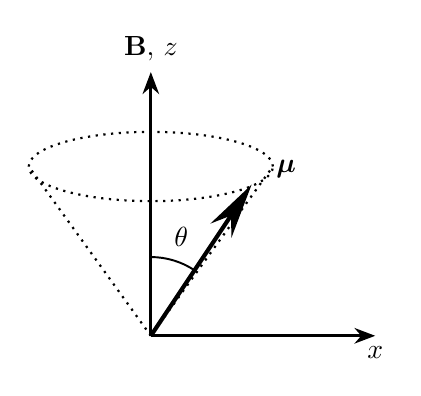
\begin{tikzpicture}[line width=0.9pt,>=Stealth]
% 竖直轴 B, z
\draw[->,line width=1.1pt] (0,0) -- (0,3.35) node[above] {$\mathbf{B},\,z$};
% 水平轴 x
\draw[->,line width=1.0pt] (0,0) -- (2.85,0) node[below] {$x$};
% 进动轨迹（点线椭圆）与锥面轮廓
\draw[dotted,line width=0.8pt] (0,2.15) ellipse (1.55 and 0.44);
\draw[dotted,line width=0.8pt] (0,0) -- (-1.55,2.15);
\draw[dotted,line width=0.8pt] (0,0) -- (1.55,2.15);
% 磁矩 mu（粗偶极针，指向锥面前沿一点）
\draw[line width=1.5pt,-{Stealth[length=7mm,width=3.2mm]}] (0,0) -- (1.28,1.92);
\node at (1.72,2.12) {$\boldsymbol{\mu}$};
% 夹角 theta
\draw[line width=0.7pt] (90:1.0) arc[start angle=90,end angle=56,radius=1.0];
\node at (73:1.32) {$\theta$};
\end{tikzpicture}
\end{document}
